\documentclass{article}\usepackage{graphicx, color}
%% maxwidth is the original width if it is less than linewidth
%% otherwise use linewidth (to make sure the graphics do not exceed the margin)
\makeatletter
\def\maxwidth{ %
  \ifdim\Gin@nat@width>\linewidth
    \linewidth
  \else
    \Gin@nat@width
  \fi
}
\makeatother

\definecolor{fgcolor}{rgb}{0.2, 0.2, 0.2}
\newcommand{\hlnumber}[1]{\textcolor[rgb]{0,0,0}{#1}}%
\newcommand{\hlfunctioncall}[1]{\textcolor[rgb]{0.501960784313725,0,0.329411764705882}{\textbf{#1}}}%
\newcommand{\hlstring}[1]{\textcolor[rgb]{0.6,0.6,1}{#1}}%
\newcommand{\hlkeyword}[1]{\textcolor[rgb]{0,0,0}{\textbf{#1}}}%
\newcommand{\hlargument}[1]{\textcolor[rgb]{0.690196078431373,0.250980392156863,0.0196078431372549}{#1}}%
\newcommand{\hlcomment}[1]{\textcolor[rgb]{0.180392156862745,0.6,0.341176470588235}{#1}}%
\newcommand{\hlroxygencomment}[1]{\textcolor[rgb]{0.43921568627451,0.47843137254902,0.701960784313725}{#1}}%
\newcommand{\hlformalargs}[1]{\textcolor[rgb]{0.690196078431373,0.250980392156863,0.0196078431372549}{#1}}%
\newcommand{\hleqformalargs}[1]{\textcolor[rgb]{0.690196078431373,0.250980392156863,0.0196078431372549}{#1}}%
\newcommand{\hlassignement}[1]{\textcolor[rgb]{0,0,0}{\textbf{#1}}}%
\newcommand{\hlpackage}[1]{\textcolor[rgb]{0.588235294117647,0.709803921568627,0.145098039215686}{#1}}%
\newcommand{\hlslot}[1]{\textit{#1}}%
\newcommand{\hlsymbol}[1]{\textcolor[rgb]{0,0,0}{#1}}%
\newcommand{\hlprompt}[1]{\textcolor[rgb]{0.2,0.2,0.2}{#1}}%

\usepackage{framed}
\makeatletter
\newenvironment{kframe}{%
 \def\at@end@of@kframe{}%
 \ifinner\ifhmode%
  \def\at@end@of@kframe{\end{minipage}}%
  \begin{minipage}{\columnwidth}%
 \fi\fi%
 \def\FrameCommand##1{\hskip\@totalleftmargin \hskip-\fboxsep
 \colorbox{shadecolor}{##1}\hskip-\fboxsep
     % There is no \\@totalrightmargin, so:
     \hskip-\linewidth \hskip-\@totalleftmargin \hskip\columnwidth}%
 \MakeFramed {\advance\hsize-\width
   \@totalleftmargin\z@ \linewidth\hsize
   \@setminipage}}%
 {\par\unskip\endMakeFramed%
 \at@end@of@kframe}
\makeatother

\definecolor{shadecolor}{rgb}{.97, .97, .97}
\definecolor{messagecolor}{rgb}{0, 0, 0}
\definecolor{warningcolor}{rgb}{1, 0, 1}
\definecolor{errorcolor}{rgb}{1, 0, 0}
\newenvironment{knitrout}{}{} % an empty environment to be redefined in TeX

\usepackage{alltt}
\IfFileExists{upquote.sty}{\usepackage{upquote}}{}


\begin{document}

\section*{Williamstown Weather}

This graph illustrates the average temperature (in degrees Celsius) of
Williamstown, Massachusetts from 1892 to 2010.

\begin{knitrout}
\definecolor{shadecolor}{rgb}{0.969, 0.969, 0.969}\color{fgcolor}\begin{kframe}
\begin{alltt}
x <- \hlfunctioncall{read.table}(\hlstring{"weather.txt"}, header = TRUE)
\hlfunctioncall{library}(lubridate)
\hlfunctioncall{library}(reshape)
\hlfunctioncall{library}(ggplot2)
y <- \hlfunctioncall{melt}(x, id = \hlstring{"Year"})
stringDates <- \hlfunctioncall{paste}(y$variable, y$Year, 20, sep = \hlstring{"/"})
Date <- \hlfunctioncall{as.Date}(stringDates, format = \hlstring{"%b/%Y/%d"})
Temperatures <- y$value
\hlfunctioncall{qplot}(x = Date, y = Temperatures, geom = \hlstring{"line"})
\end{alltt}
\end{kframe}
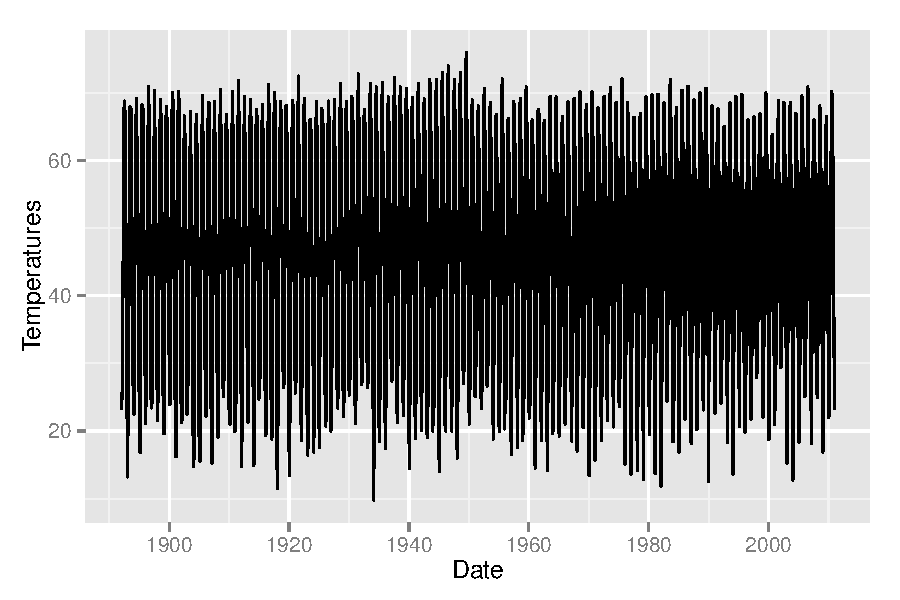
\includegraphics[width=\maxwidth]{figure/graph1} 

\end{knitrout}


This graph illustrates the average daily temperatures in degrees Celsius of
Williamstown, Massachusetts from 2005 to 2013.

\begin{knitrout}
\definecolor{shadecolor}{rgb}{0.969, 0.969, 0.969}\color{fgcolor}\begin{kframe}
\begin{alltt}
x <- \hlfunctioncall{read.table}(\hlstring{"link1.txt"})
dates1 <- x[, 1]
temps1 <- x[, 3]
\hlfunctioncall{plot}(dates1, temps1, xlab = \hlstring{"Date"}, ylab = \hlstring{"\hlfunctioncall{Temperature} (degrees Celsius)"})
\end{alltt}
\end{kframe}
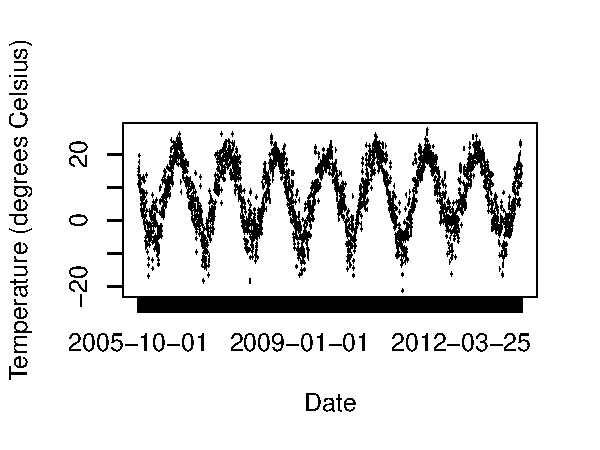
\includegraphics[width=\maxwidth]{figure/graph2} 

\end{knitrout}


This graph illustrates the average daily temperatures in degrees Celsius of
Williamstown, Massachusetts from 1983 to 2007.

\begin{knitrout}
\definecolor{shadecolor}{rgb}{0.969, 0.969, 0.969}\color{fgcolor}\begin{kframe}
\begin{alltt}
y <- \hlfunctioncall{read.table}(\hlstring{"link2.txt"}, sep = \hlstring{"\textbackslash{}t"})
dates2 <- y[, 1]
temps2 <- y[, 2]
\hlfunctioncall{plot}(dates2, temps2, xlab = \hlstring{"Date"}, ylab = \hlstring{"\hlfunctioncall{Temperature} (degrees Celsius)"})
\end{alltt}
\end{kframe}
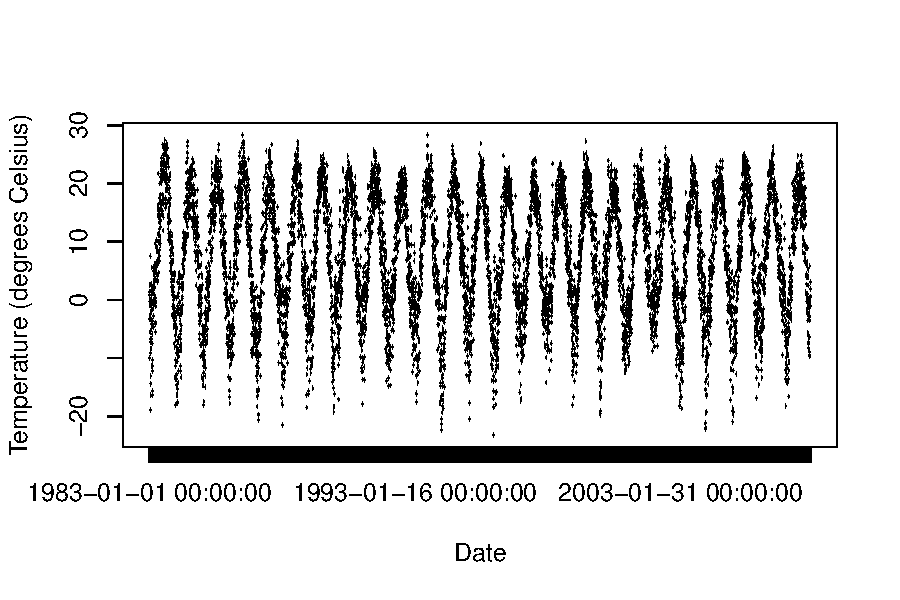
\includegraphics[width=\maxwidth]{figure/graph3} 

\end{knitrout}


\end{document}
